\begin{figure}[t]
\vspace*{-2ex}
\centering
\begin{subfigure}{.18\textwidth}
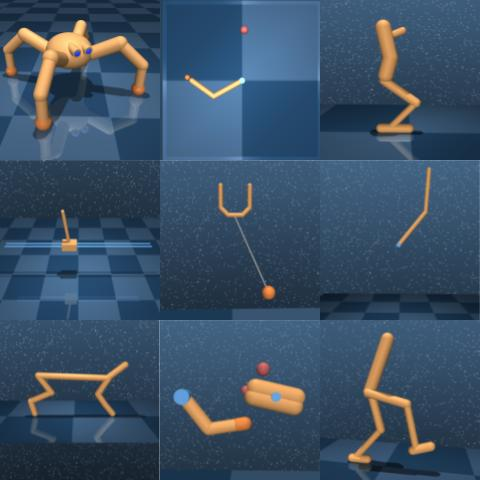
\includegraphics[width=\linewidth]{tasks/dmc}
\caption{控制套件}
\end{subfigure}\hfill
\begin{subfigure}{.18\textwidth}
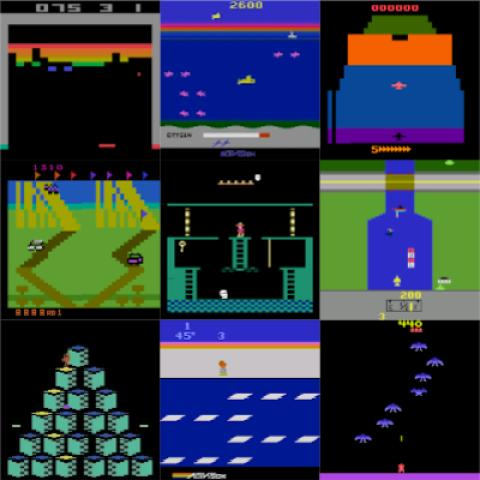
\includegraphics[width=\linewidth]{tasks/atari}
\caption{Atari}
\end{subfigure}\hfill
\begin{subfigure}{.18\textwidth}
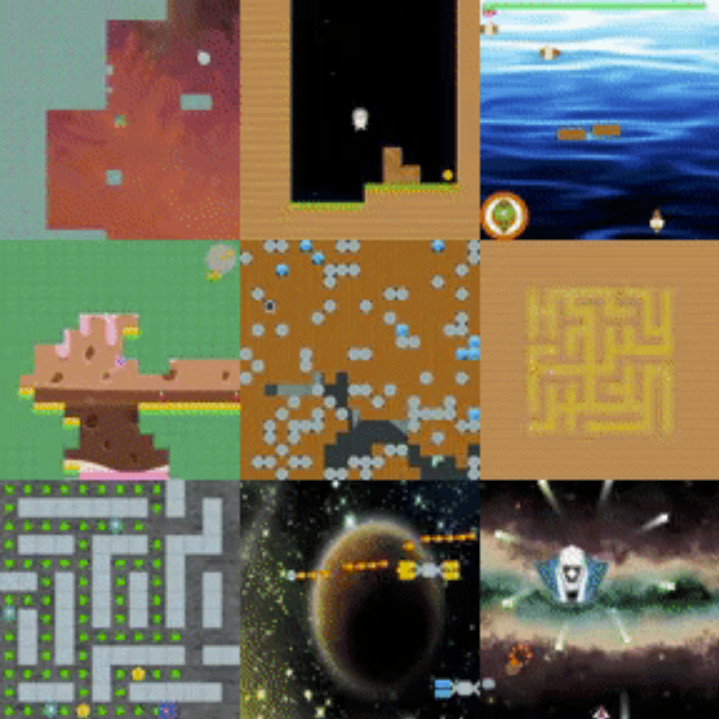
\includegraphics[width=\linewidth]{tasks/procgen}
\caption{ProcGen}
\end{subfigure}\hfill
\begin{subfigure}{.18\textwidth}
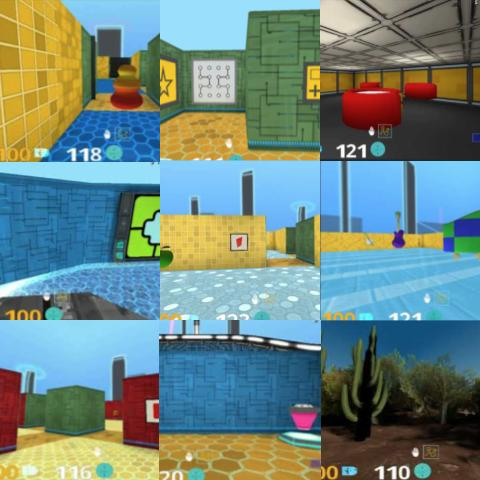
\includegraphics[width=\linewidth]{tasks/dmlab}
\caption{DMLab}
\end{subfigure}\hfill
\begin{subfigure}{.18\textwidth}
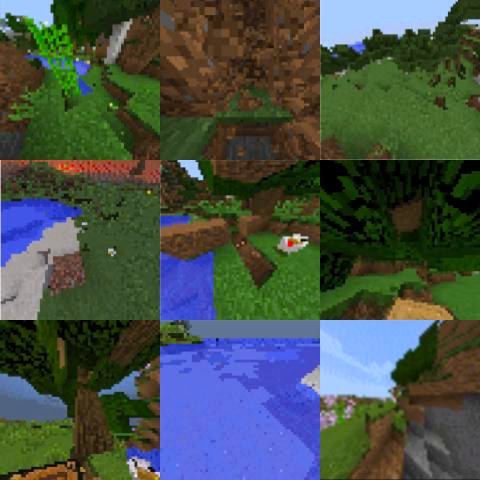
\includegraphics[width=\linewidth]{tasks/minecraft}
\caption{Minecraft}
\end{subfigure}
\caption{实验中使用的多样化视觉领域。Dreamer 能在这些领域中取得成功，覆盖机器人运动和操作任务、Atari 游戏、程序生成的 ProcGen 关卡、需要空间和时间推理的 DMLab 任务，以及复杂且无限的 Minecraft 世界。我们也在非视觉领域上评估 Dreamer。}
\label{fig:tasks}
\end{figure}
